\chapter[Metodologia]{Metodologia}
\label{cp:metodologia}

\begin{figure}[H]
	\centering
	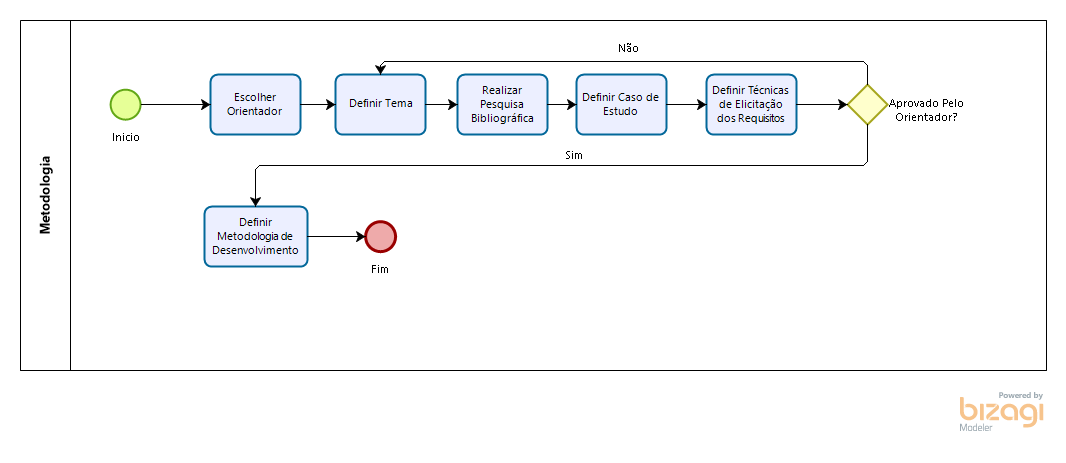
\includegraphics[width=1.0\textwidth]{figuras/metodologia.png}
	\caption{Metodologia. Fonte: Própria}
	\label{img:metodologia}
\end{figure}

A figura \ref{img:metodologia} mostra como foi elaborada a metodologia deste projeto. Alguns processos demonstrados já foram elaborados como "Escolher o Orientador, Definir Tema" e "Realizar Pesquisa Bibliográfica". A seguir, os demais processos serão contemplados e explicados adequadamente.

\section{A Instituição}

Tendo a justificativa para o projeto no tópico \ref{sec:justificativa}, seguida do problema de pesquisa (\ref{sec:problema_de_pesquisa}) e os objetivos descritos no tópico \ref{sec:objetivos}, houve a necessidade de escolher alguma empresa que seria usada como caso de estudo para o projeto, no caso foi definido o NMIL (Núcleo de Modernização da Informação Legislativa), um setor localizado no Senado Federal Brasileiro.

\subsection{Senado Federal}

As funções do Senado Federal são exercidas pelos senadores da República, que são eleitos segundo o princípio majoritário para representarem os estados e o Distrito Federal. Os estado e o Distrito Federal elegem três senadores para um mandato de oito anos. A renovação da representação se dá a cada quatro anos, alternadamente, por um e dois terços. Cada senador é eleito com dois suplentes.

A Estrutura Administrativa compreende a formação das unidades do Senado, suas
atribuições, responsáveis e formas de contato.

A Administração tem como ênfase os compromissos com o Parlamento; com excelência na prestação de serviços públicos; com qualidade de vida dos colaboradores; com a igualdade; com a livre disseminação de ideias; com a transparência; com a responsabilidade na utilização
de recursos públicos; com a memória do Senado; e com a comunidade. Na figura \ref{img:organograma_senado} pode ser visualizado o organograma organizacional do Senado Federal com suas casas e secretárias.

\begin{figure}[H]
	\centering
	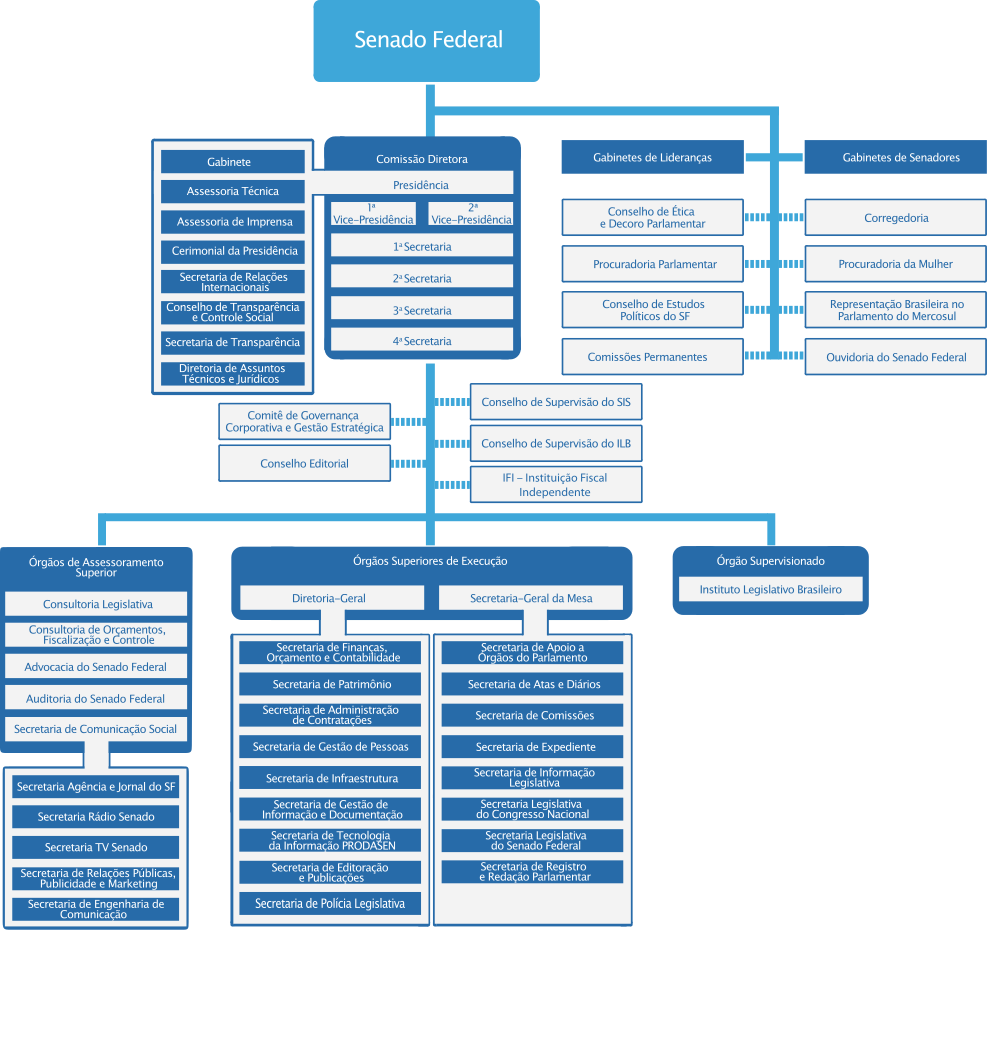
\includegraphics[width=0.8\textwidth]{figuras/organograma_senado.png}
	\caption{Organograma Senado Federal. Fonte: \citeonline{organograma_senado}.}
	\label{img:organograma_senado}
\end{figure}

\subsection{NMIL}

A Comissão Diretora é composta pelo Presidente, dois Vice-Presidentes e quatro
Secretários. A composição dessa comissão muda a cada dois anos, sendo assim na primeira e terceira fase de uma legislatura, sendo esta com duração de 4 anos. É de responsabilidade da Comissão a direção da casa, designando atividades às unidades que dão suporte.

Essas unidades são: Secretaria Geral da Mesa (SGM), representante da atividade fim da casa; e Diretoria Geral (DGER), que, representa as atividades meio da casa. As duas contam com secretarias, às quais delegam atividades exigidas pelo Presidente.

Quando o Presidente da Comissão Diretora necessita de apoio tecnológico, delega esta
atividade à SGM, que, ao receber o problema, começa a definir diretrizes estratégicas para a solução do problema. Após o término da definição das diretrizes, encaminha-as à Secretaria de Informação Legislativa (Sinfleg).

O diretor da Sinfleg atua como Gerente do Projeto, e conta com o apoio da equipe do
NMIL na administração do projeto.

A equipe do NMIL realiza reuniões com as áreas afetadas pelo projeto até conseguir
definir todos os requisitos para o produto que será gerado. Após a definição, convoca uma reunião com o Gerente para entrega dos requisitos definidos. O Gerente analisa esses requisitos para saber se são viáveis. Caso não sejam, pede ao NMIL novos requisitos e, só após receber requisitos viáveis, aprova a proposta de solução.

O próximo passo é dado pelo NMIL, convocando reunião com a Secretaria de Tecnologia da Informação (Prodasen). Nesta reunião discute-se os requisitos aprovados e prepara-se o Termo de Abertura do Projeto (TAP). O TAP, deve ser encaminhado pelo NMIL ao Gerente para que este aprove o documento; caso não aprove, pede-se um novo, até que seja aprovado.

Após o Gerente aprovar o projeto, ele o apresenta ao Secretário Geral da Mesa, que é o representante da SGM, para uma aprovação final. O Secretário Geral da Mesa também pode pedir um novo projeto, mas se não for o caso, apenas o autoriza.

Dada a aprovação do Secretário Geral da Mesa, a equipe do Prodasen, responsável pela
construção do produto, dá início à construção do projeto, fazendo as entregas de ambiente de homologação (definidas no TAP) ao NMIL, a fim de que este realize testes. Se forem encontrados erros, estes são listados e repassados ao Prodasen para que sejam reparados. Quando não há mais erros, o NMIL dá sua aprovação do produto. Em seguida o Prodasen termina sua parte do projeto e entrega o produto finalizado ao NMIL. O NMIL encaminha o produto ao
Gerente que autoriza o produto e apresenta-o ao Secretário Geral da Mesa.

O Secretário Geral da Mesa, após receber o produto, pode solicitar alterações ao NMIL,
que em seguida encaminha esta solicitação ao Prodasen. A equipe do Prodasen responsável pelo produto faz as alterações necessárias o encaminha de volta ao NMIL, passando pelo processo de teste e aprovação novamente até que o Secretário Geral da Mesa autorize a implantação.

Quando o Secretário Geral da Mesa autorizar a implantação, cabe ao NMIL apresentar
aos usuários o novo Sistema ou as atualizações em sistemas já existentes.

As figuras relacionadas ao mapeamento do processo que ocorre atualmente no NMIL, pode ser vistos no apêndice \ref{ch:figuras}, sendo as figura \ref{img:modelagemProcessoGeral1Parte1} e \ref{img:modelagemProcessoGeral1Parte2} como o processo de pedido da comissão diretora para um novo sistema passando pela SGM, Sinfleg, NMIL e por fim ao Prodasen. As figuras \ref{img:modelagemProcessoGeral2Parte1} e \ref{img:modelagemProcessoGeral2Parte2} se referem ao processo que o NMIL passa até conseguir atingir um sistema estável e que atenda ao pedida da comissão diretora.

\section{Metodologia de Desenvolvimento}

Por conta de possuir um maior conhecimento sobre a metodologia e pela proposta em entregas mais frequentes em períodos menores, foi escolhida a metodologia ágil \textit{Scrum}, explicada no tópico \ref{sec:modelo_agil} como metodologia de desenvolvimento do \textit{software} juntamente com algumas práticas do \textit{Scrum} Solo. 

\subsection{Scrum}

Uma das principais vantagens do \textit{Scrum} é a adaptação dele a projetos menores e que não são rigorosos a processos, e após ser feita uma análise dos tipos de gerenciamento de projetos no tópicos \ref{sec:gerenciamento_de_projetos}, foi escolhido o \textit{Scrum} Solo como adaptação do \textit{framework Scrum} como metodologia de desenvolvimento deste TCC.

\subsubsection{Papéis}

Este projeto será desenvolvido de forma individual, os papéis do \textit{framework} \textit{Scrum} foram distribuídos de forma com que cada ator tenha a seguinte responsabilidade: o responsável pelo desenvolvido do sistema, Victor Mota, assume os papéis de Time de Desenvolvimento e \textit{Scrum Master}. O papel de \textit{Product Owner} será assumido por Pedro Marques, servidor do Senado Federal e do NMIL, que é o setor de caso de estudo deste trabalho. 

\subsubsection{Sprints}

Para este projeto, as \textit{Sprints} foram definidas com duração máxima de duas semanas. Assim como define no \textit{Scrum}, as \textit{Sprints} devem ter as atividades de planejamento e revisão da mesma, para que seja constatado se o que foi planejado foi entregue ao longo das duas semanas.

\begin{itemize}
    \item \textit{Sprint Planning}: Esta atividade é realizada no primeiro dia de \textit{Sprint} e é nela que são selecionados os itens do \textit{Product Backlog} que serão desenvolvidos ao longo da \textit{Sprint};
    \item \textit{Sprint Review}: Esta atividade é realizada no último dia de \textit{Sprint} e é nela são discutidas com \textit{Product Owner} as histórias de usuário desenvolvidas ao longo da \textit{Sprint}.   
\end{itemize}